%======================================================================
\subsection{BW-SIM-07 plan: a COMSOL/Ansys-style simulation workspace (31 Oct 2026)}\label{sec:sim07-plan}
%======================================================================

You asked for the simulation setup to look and work like COMSOL or Ansys rather than like an open-source tool, and
chose both a COMSOL-style model builder and an Ansys-style project schematic. This plan shows the workspace today,
the proposed one in three mockups, how it maps onto the objects we already have, and the questions to settle before
code.

%----------------------------------------------------------------------
\subsubsection*{Today}

Figure~\ref{fig:simui-today} is the GUI build after solving a plate with a hole. An agent walked through every step
with off-screen screenshots and read the code (\file{bruceworx\_sim\_gui.py}, \file{bruceworx\_cfd\_gui.py}).
What it found:
\begin{itemize}[nosep]
  \item \textbf{Settings in three places.} Study type, part, material and mesh size are set once in the \emph{New
        Study} panel. Loads open FreeCAD's stock constraint panels. Everything else is in sections of one long
        study panel. Material and mesh size cannot be edited later as nodes of their own.
  \item \textbf{The tree shows one collapsed ``Study'' object.} There are no ordered steps (geometry, materials,
        physics, mesh, study steps, results), and selecting something does not show its settings.
  \item \textbf{Buttons that close and reopen the panel.} \emph{+ Force} closes the study panel, opens the stock
        panel, and reopens the study panel afterwards, losing the scroll position.
  \item \textbf{No messages, progress or log pane.} A solve reports ``Solved in 0.7\,s'' and nothing else; the
        results sit below the fold and need scrolling.
  \item \textbf{Different layouts.} Airflow studies use their own form and have no list of boundary conditions.
        The ribbon shows about 35 buttons whatever the study type, most of them greyed.
\end{itemize}

\begin{figure}[h]
\centering
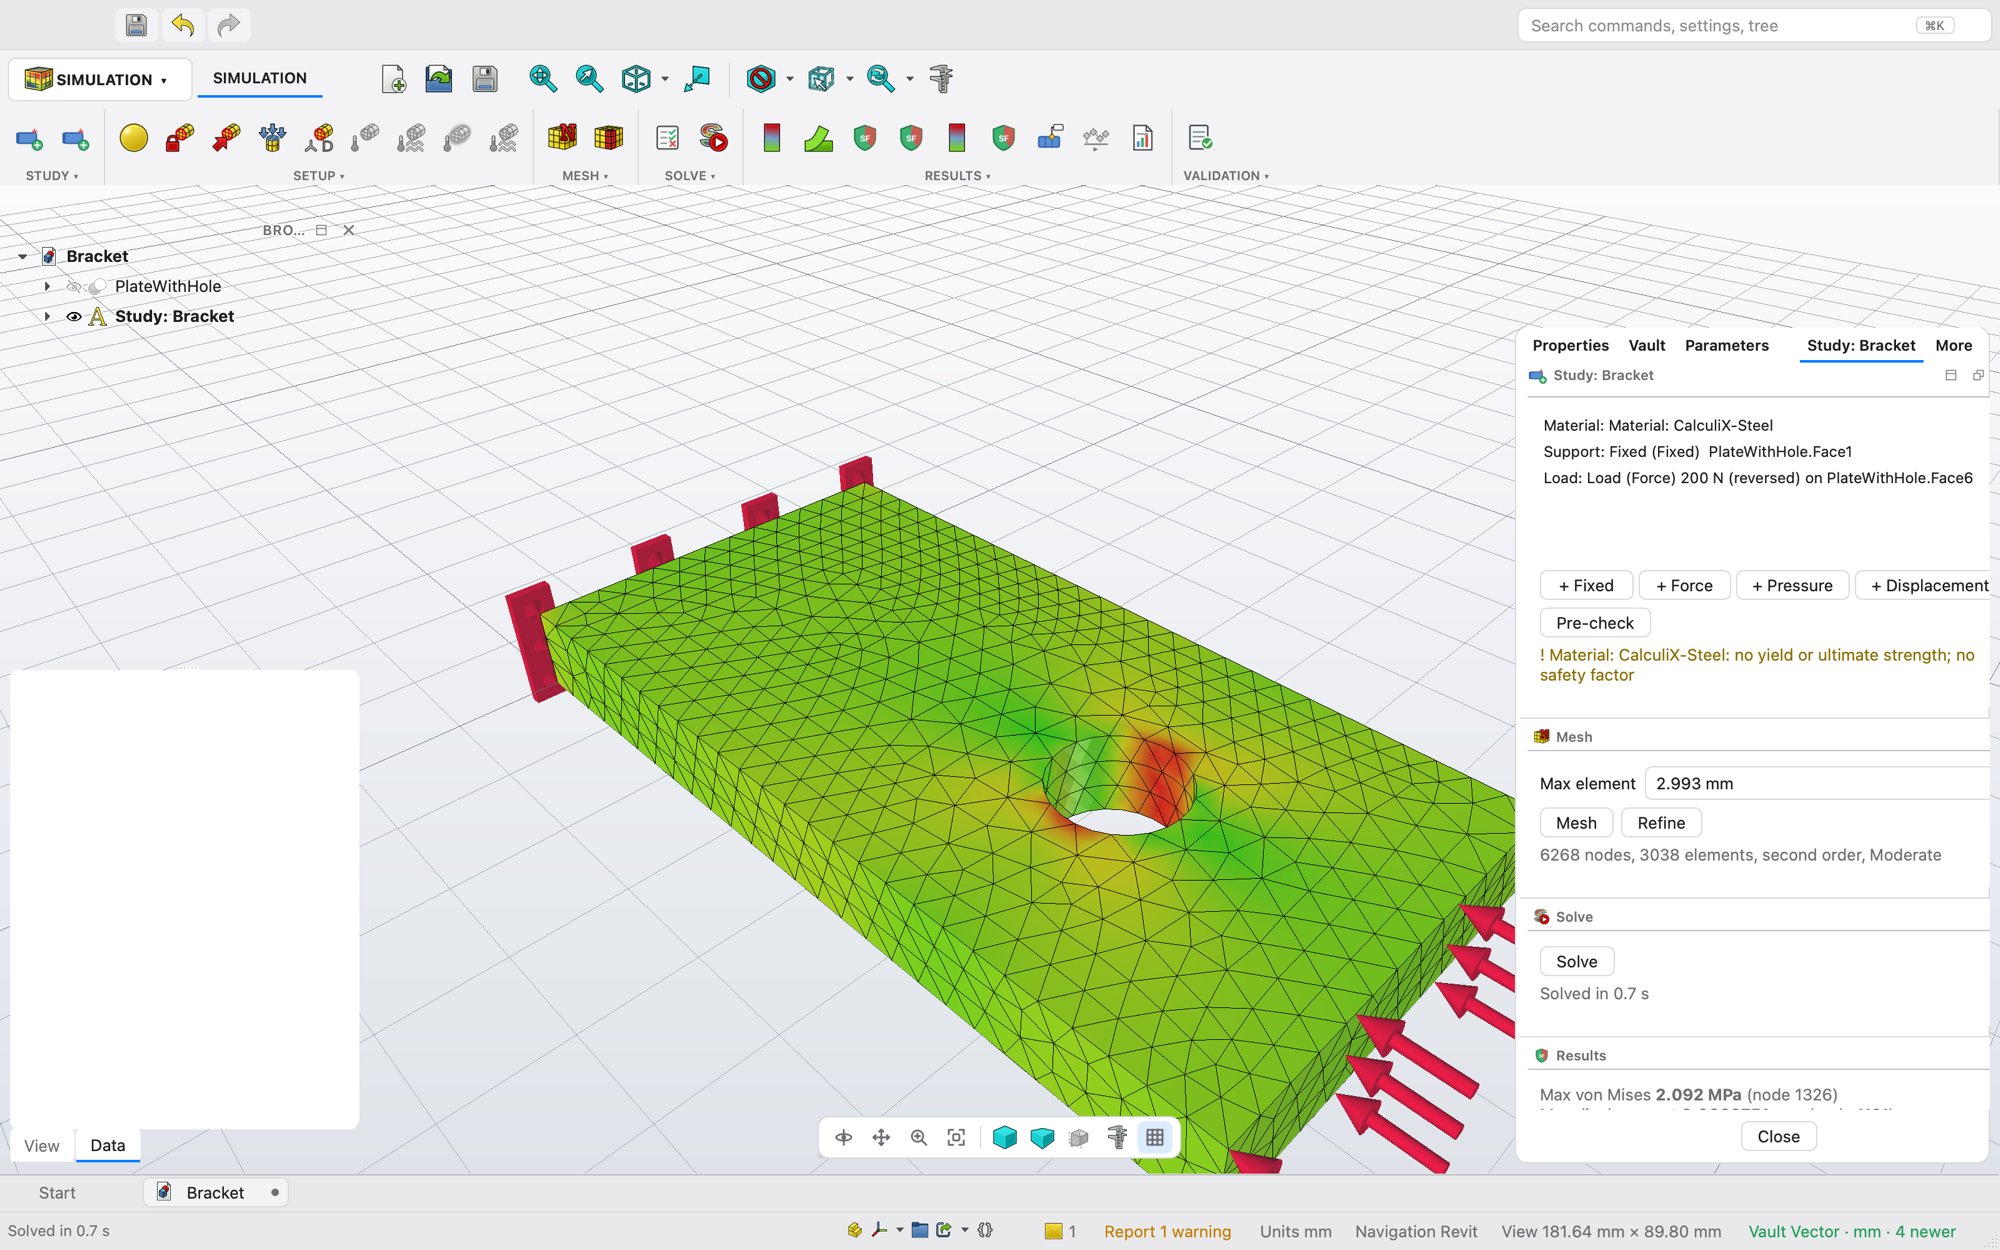
\includegraphics[width=\linewidth]{fig/simui_today_solved.png}
\caption{Today: a solved static study. The study is one object in a small tree (left), the settings are one long
panel on the right, the results are below its fold, and there is no messages or progress pane.}
\label{fig:simui-today}
\end{figure}

%----------------------------------------------------------------------
\subsubsection*{The proposed workspace}

\paragraph{Model builder (Fig.~\ref{fig:simui-setup}).} Four panes, as in COMSOL Multiphysics:
\begin{description}[nosep,font=\normalfont\bfseries]
  \item[Model Builder] (left): one tree for the whole study, in solving order: Global Definitions (parameters,
        named selections), Geometry, Materials, Physics (supports, loads, contacts; boundary conditions for
        airflow), Mesh, Study (steps and solver) and Results (plots, probes, graphs, reports). Each node shows its
        state on the right: up to date, out of date, needs attention, running, or not set up.
  \item[Settings] (middle): the settings of the selected node, in folding sections (Label, Selection, Force,
        \ldots). Faces are added or removed by clicking in the graphics while the node is selected, so the panel
        never closes. Every numeric field takes an expression with a unit and parameters (\code{F\_load},
        \code{2*t+1[mm]}).
  \item[Graphics] (right): the model, with the selection highlighted, load arrows and support hatching, a
        light-blue gradient background, an axis triad, and the legend and max/min labels for results.
  \item[Messages, Progress, Log, Table] (below the graphics): pre-check findings with times, a bar per stage of a
        run (mesh, write, solve, load results), the solver's own output, and tables of evaluated values.
\end{description}
The ribbon gets one tab per step: Home, Definitions, Geometry, Materials, Physics, Mesh, Study, Results, Project.
Each shows only the commands that fit the current study type: a prop-wash study has no \emph{Pressure} button and a
static study has no \emph{Inlet}.

\begin{figure}[h]
\centering
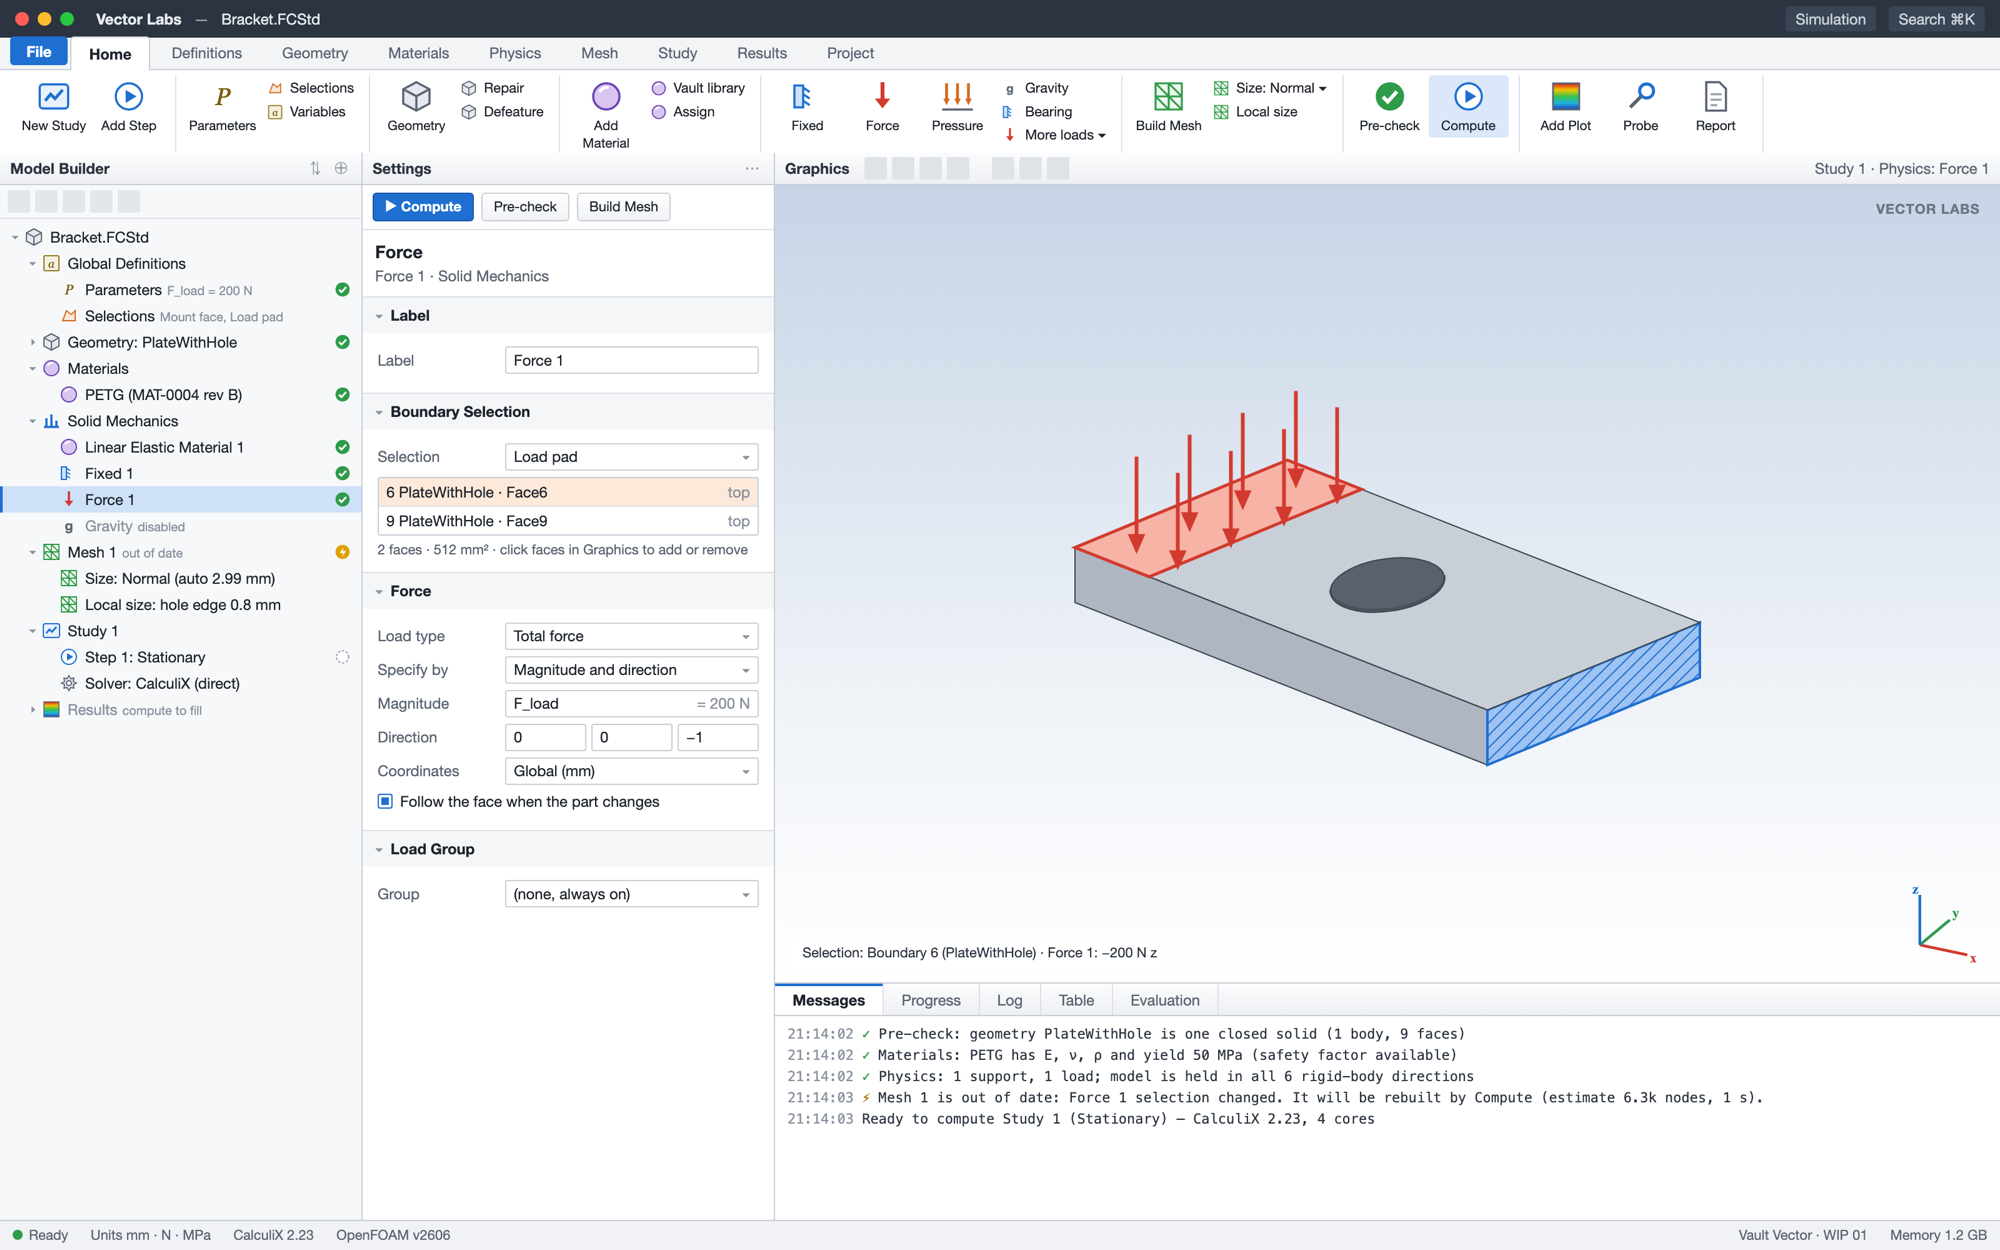
\includegraphics[width=\linewidth]{fig/simui_m1_setup.png}
\caption{Mockup: setting up a static study. \emph{Force 1} is selected in the Model Builder; its settings take a
parameter for the magnitude, and its two faces are listed and highlighted in red in the graphics. The mesh is
marked out of date because the selection changed; \emph{Compute} rebuilds it.}
\label{fig:simui-setup}
\end{figure}

\begin{figure}[h]
\centering
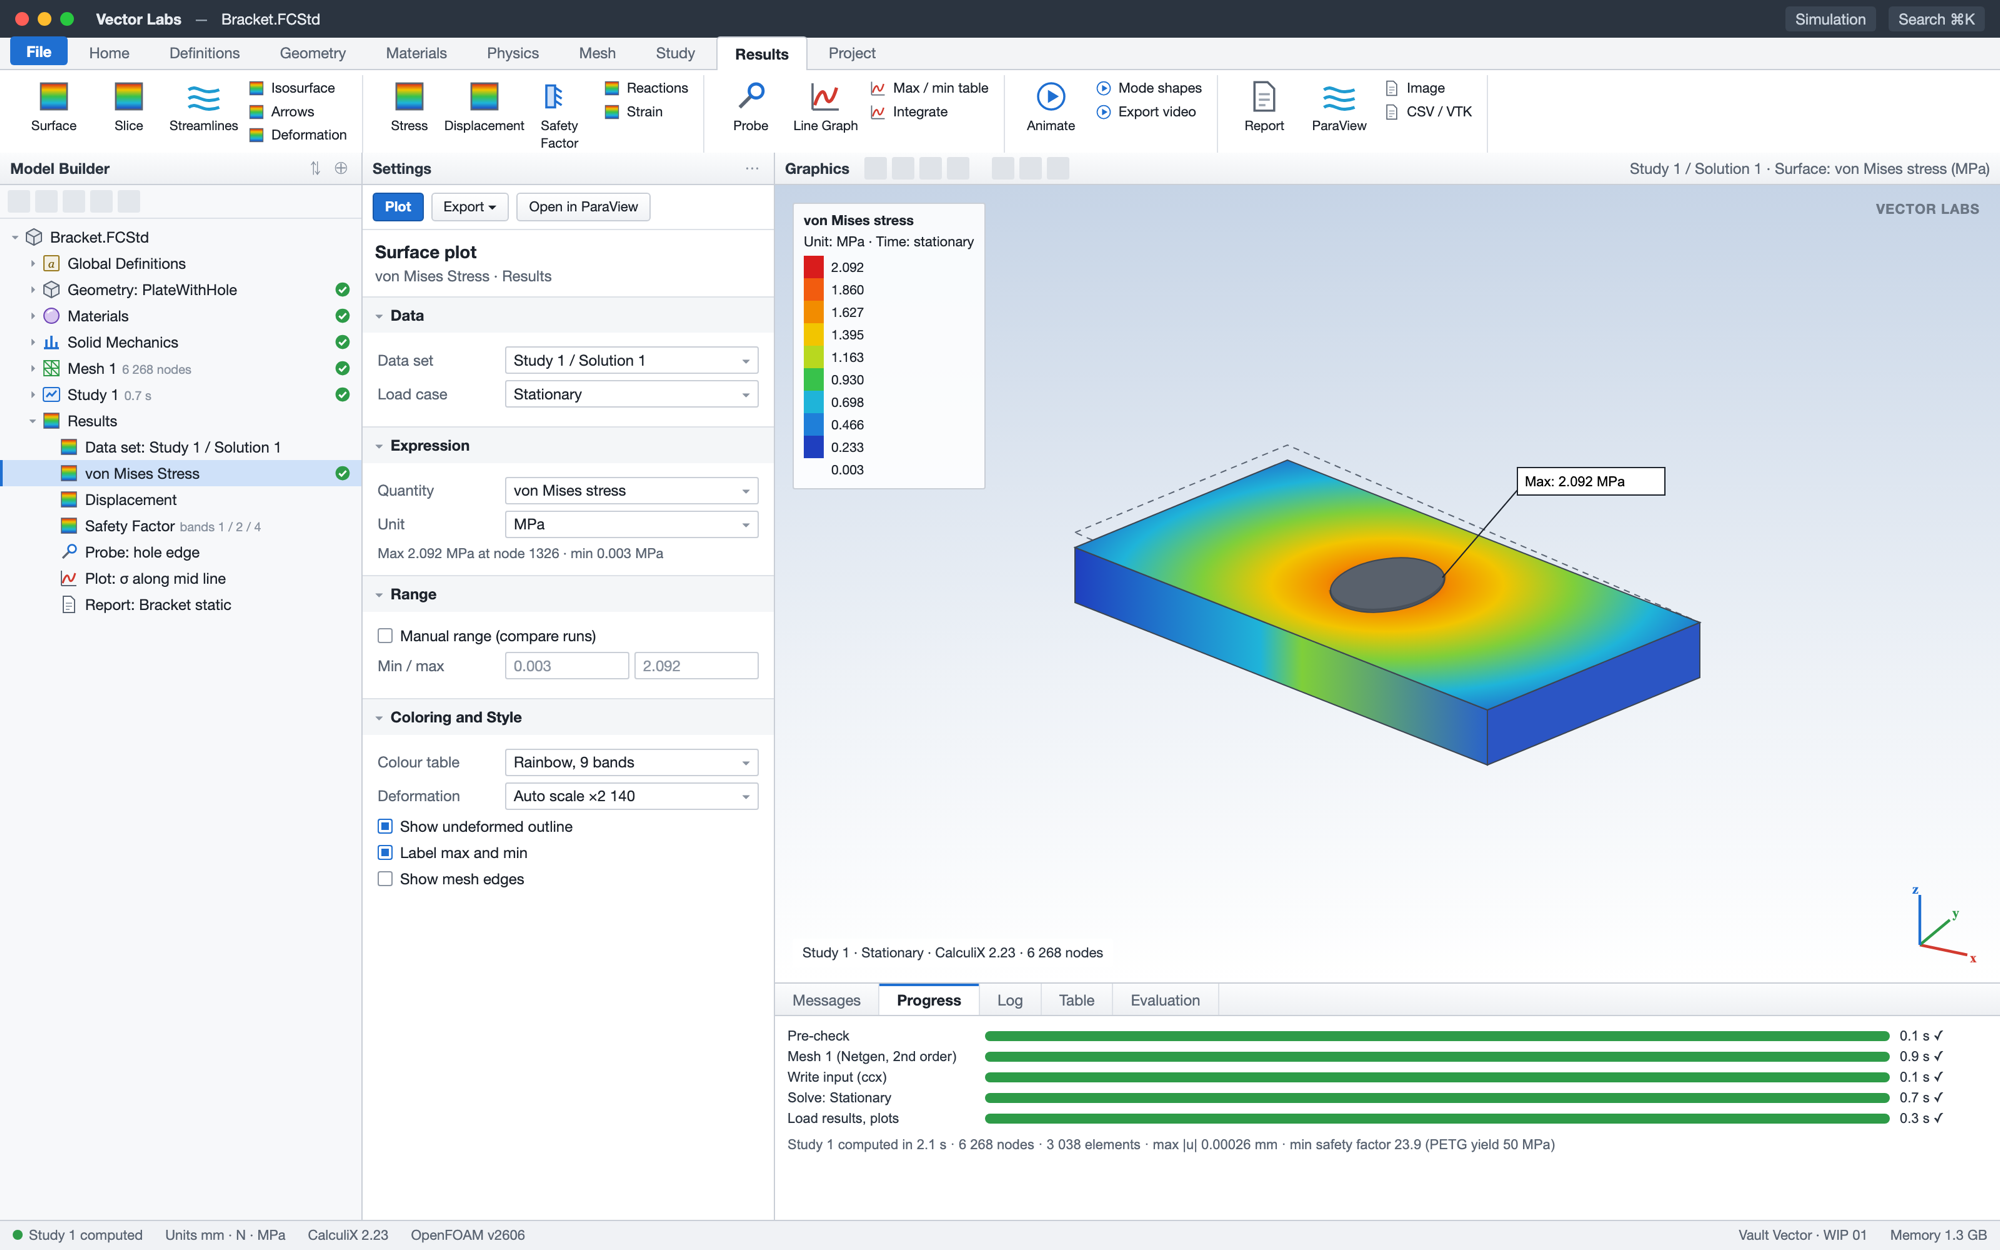
\includegraphics[width=\linewidth]{fig/simui_m2_results.png}
\caption{Mockup: results. Each plot is a node under Results with its own settings (data set, quantity, unit,
range, colour table, deformation). The Progress tab shows each stage of the run with its time.}
\label{fig:simui-results}
\end{figure}

\paragraph{Project schematic (Fig.~\ref{fig:simui-project}).} A page that shows every study in the document as a
block of cells, as in Ansys Workbench: engineering data, geometry, model or mesh, setup, solution and results. A
line between two blocks shares data. A plain line shares geometry or materials; an orange line transfers results, for
example the wall pressure of a prop-wash study becoming a load on a static study of the arms. Each cell has the same
state mark as its node in the Model Builder. \emph{Update Project} solves everything out of date, in the right
order, within a core budget. Double-clicking a cell opens that node in the Model Builder.

\begin{figure}[h]
\centering
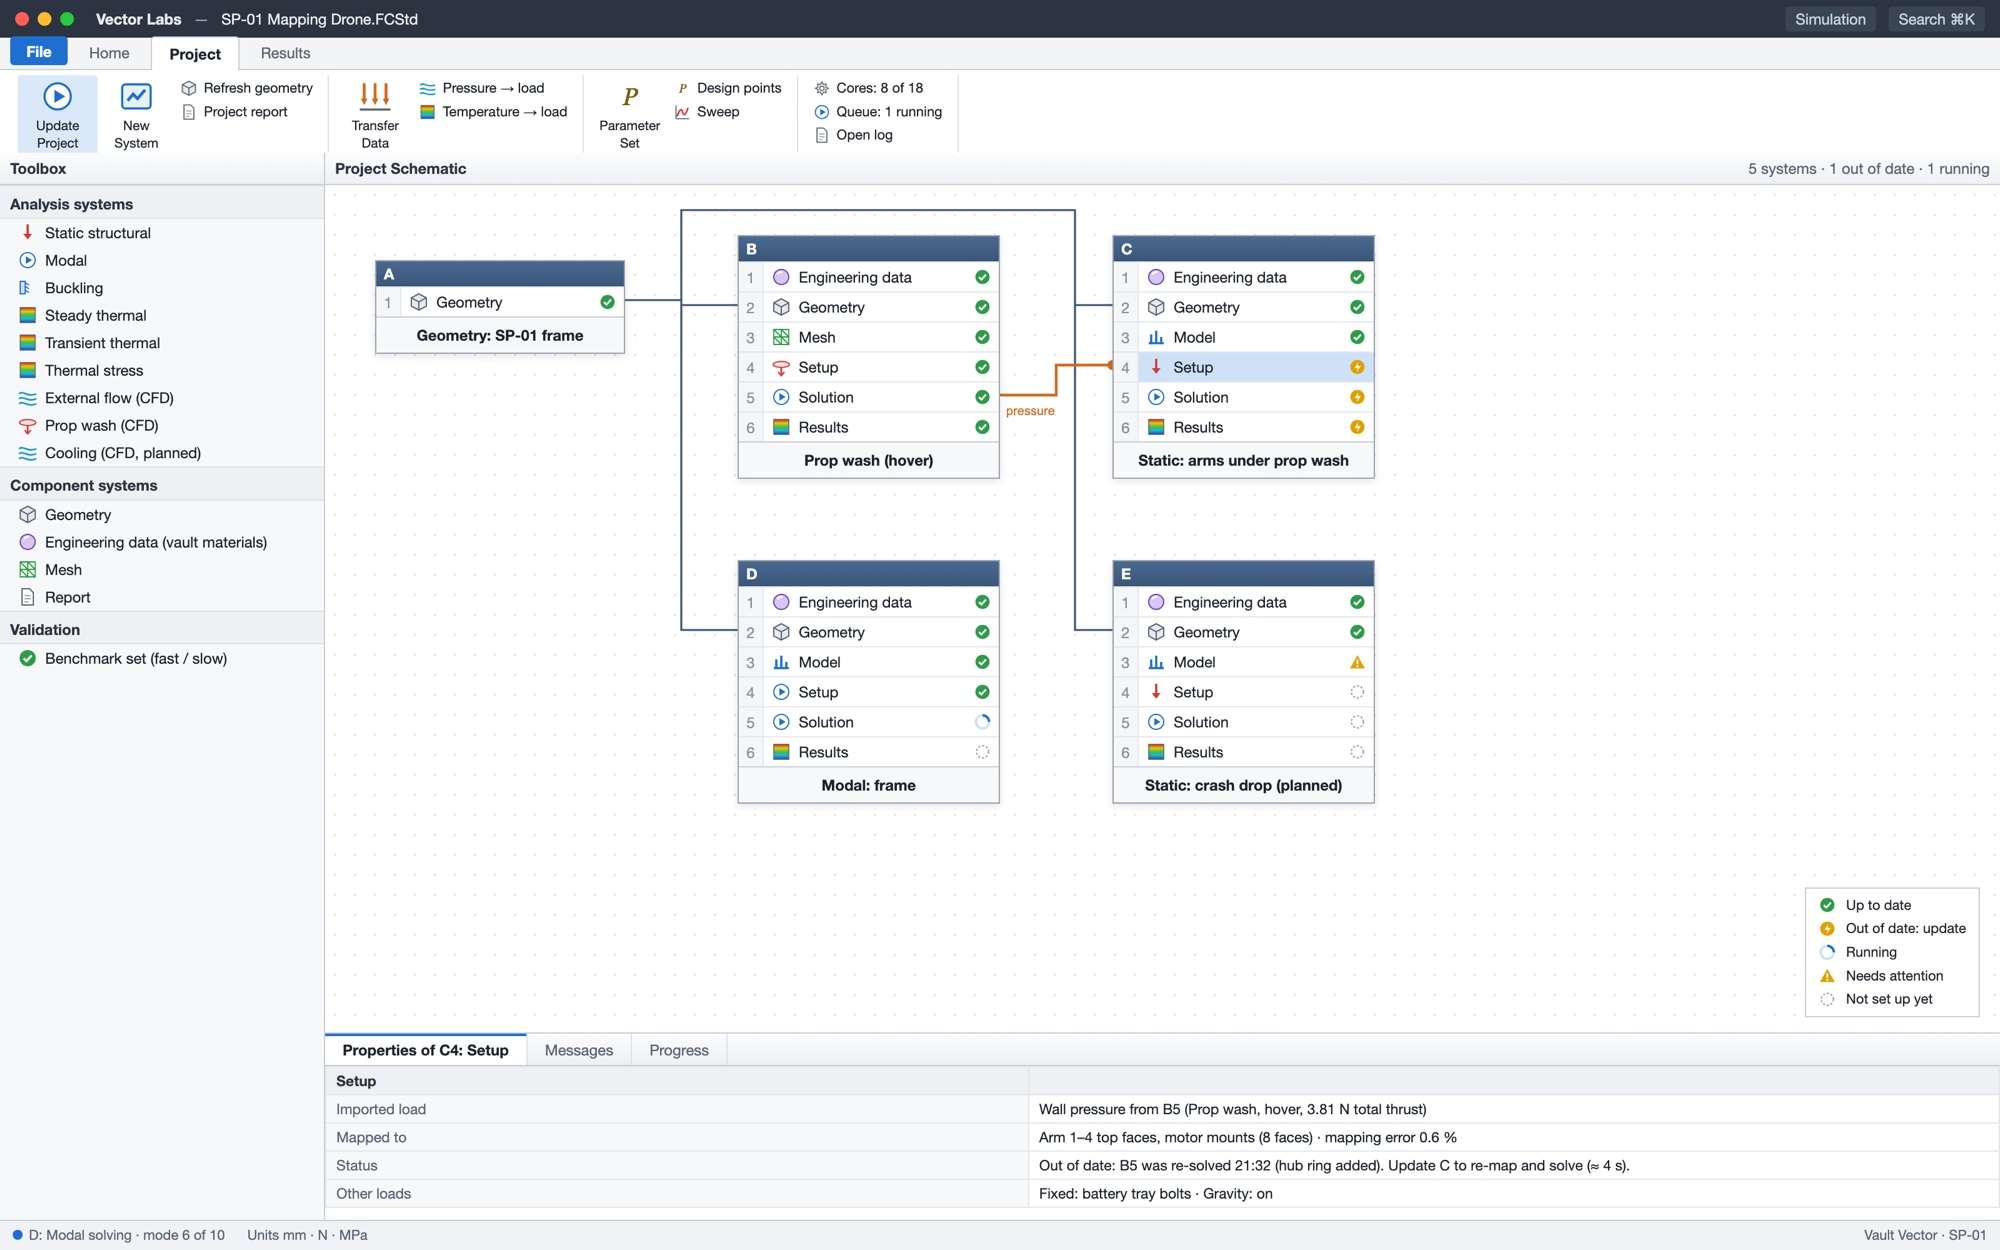
\includegraphics[width=\linewidth]{fig/simui_m3_project.png}
\caption{Mockup: the project schematic for SP-01. The prop-wash study (B) was solved again after the hub ring was
added, so the static study of the arms (C), which takes B's wall pressure as its load, is out of date from its
setup down. The modal study (D) is running.}
\label{fig:simui-project}
\end{figure}

%----------------------------------------------------------------------
\subsubsection*{How it works}

\paragraph{A view over the objects we have.} The solvers do not change. CalculiX and OpenFOAM still get their input
from the FEM analysis and its children. The Model Builder is a new tree widget that shows those objects in solving
order, plus a few new ones:
\begin{center}
\small
\begin{tabularx}{\linewidth}{@{}lX@{}}
\toprule
Node & Stored as\\
\midrule
Parameters & a parameter table on the study (name, expression, value, unit); loads and mesh sizes refer to them\\
Selections & new \emph{named selection} objects: a list of faces, edges or bodies that survives model changes
             (the same topological-naming repair as loads)\\
Materials & FEM material objects, linked to the vault material by number and revision\\
Physics & FEM constraints, and the airflow boundary conditions as their own objects\\
Mesh & the mesh object and new \emph{local size} children\\
Study steps & new \emph{step} objects (stationary, eigenfrequency, buckling, time dependent, steady CFD), so one
              study can be a preload followed by a modal step\\
Results & new plot objects (surface, slice, streamlines, arrows, isosurface, probe, line graph, report), each
          with its own settings and its own place in the tree\\
\bottomrule
\end{tabularx}
\end{center}
Studies made today open in the new workspace unchanged: their properties become nodes when the study is loaded.

\paragraph{Up-to-date tracking.} Each node keeps a fingerprint: a hash of its own settings and of the fingerprints
of the nodes it depends on,
\[
  h(n)=H\bigl(\,s(n),\;h(m_1),\dots,h(m_k)\,\bigr),\qquad m_i\in\operatorname{deps}(n),
\]
where $s(n)$ is the node's own settings and, for geometry, the shape's hash. A node is up to date when its stored
fingerprint matches the current one. Changing a face selection therefore marks the load, the mesh (when it is
refined there), the solution and every plot as out of date, and nothing upstream. \emph{Compute} and
\emph{Update Project} walk the dependency graph in topological order and rebuild only the stale nodes. Links
between studies in the schematic are edges of the same graph, so one engine marks both views.

\paragraph{One settings engine.} Each node type declares its settings once: sections, fields, units, allowed
selection type, and which fields show for which study type. The Settings pane is built from that declaration. All
study types then share one layout, the forms can be tested headless, and adding a boundary condition means writing
a declaration, not a panel.

\paragraph{Runs stream into the panes.} The CalculiX and OpenFOAM runners already have stages and logs; they would
send events (stage started or finished, residuals, warnings) to the Progress and Log tabs, and pre-check findings
to Messages. A run never blocks the window, and a second study can be queued.

\paragraph{The look.} One stylesheet for the workspace, a new set of about 40 icons drawn for it (the mockups use
first versions), status marks on nodes and cells, a gradient viewport with the triad and legend drawn in the 3D
view, and a compact density like COMSOL and Ansys: 21\,px tree rows and 22\,px fields. Results use the colour bar
fixed in \S\ref{sec:sim06-post-built}, and ParaView stays one click away (\emph{Open in ParaView}, with streamlines
and background pictures).

%----------------------------------------------------------------------
\subsubsection*{Phases}

\begin{enumerate}[nosep,label=P\arabic*.]
  \item \textbf{Shell.} The four panes and the step ribbon in the Simulation workspace; the Model Builder over the
        existing objects; Settings for the existing node types (study, material, supports, loads, mesh, solver);
        Messages, Progress and Log fed by today's runners. Existing studies open unchanged.
  \item \textbf{Definitions and steps.} Parameters with units, named selections, local mesh sizes, and study
        steps, including a preload followed by a modal step.
  \item \textbf{Results nodes.} Surface, slice, arrows, deformation, probe and line graph as nodes; streamlines
        for airflow; the report as a node that collects the plots under it.
  \item \textbf{Project schematic.} Systems, shared geometry and materials, \emph{Update Project} with a core
        budget, and the first two transfers: CFD wall pressure to a static load, and temperature to a thermal-stress
        load.
  \item \textbf{Finish.} The full icon set, a dark theme, and parameter sweeps (design points) if you want them.
\end{enumerate}
Each phase ends with a GUI acceptance run from screenshots, like the one used for this plan.

%----------------------------------------------------------------------
\subsubsection*{Questions for you}
\begin{enumerate}[label=W\arabic*.]
  \item \textbf{Own tree.} In the Simulation workspace, the Model Builder replaces FreeCAD's model tree (still one
        click away), rather than adding study nodes to the model tree. \emph{Recommendation:} yes. The model tree
        shows parts and features, not steps in solving order.
  \item \textbf{Layout.} Three columns (tree, settings, graphics) as in COMSOL, stacking the tree above the
        settings on screens narrower than 1500\,px, as in Ansys Mechanical's Outline and Details.
        \emph{Recommendation:} yes.
  \item \textbf{Ribbon.} One tab per step, showing only the commands for the current study type.
        \emph{Recommendation:} yes.
  \item \textbf{Parameters and named selections.} Fields take expressions with units and parameters, and a
        selection can be named and reused by several loads. \emph{Recommendation:} yes, in P2.
  \item \textbf{Study steps.} A study can hold several steps (preload then modal, thermal then stress).
        \emph{Recommendation:} yes, in P2. It replaces the separate thermal-stress study type.
  \item \textbf{Recompute.} Changes only mark nodes out of date, and nothing solves until you press
        \emph{Compute} or \emph{Update Project}, as in COMSOL and Ansys. \emph{Recommendation:} yes.
  \item \textbf{Schematic scope.} One schematic per document, with the studies in it; links made by dragging one
        cell onto another; the first transfers are CFD pressure to a static load and temperature to stress.
        \emph{Recommendation:} yes, in P4.
  \item \textbf{Design points.} Parameter sweeps in the schematic (for example the arm thickness from 3 to 6\,mm
        and the stress at each). \emph{Recommendation:} later, in P5.
  \item \textbf{Theme.} The light theme of the mockups first, matching the rest of Vector Labs, and a dark theme in
        P5. \emph{Recommendation:} yes.
  \item \textbf{Old panels.} When P1 passes your acceptance, the old study panels are removed rather than kept
        behind a setting. \emph{Recommendation:} remove them; two ways to do one thing doubles the testing.
  \item \textbf{Order against other work.} P1--P3 before SIM-06's cooling study and the CFD validation cases, so
        those are built straight into the new workspace. \emph{Recommendation:} yes.
\end{enumerate}

\paragraph{Your answers (1 Nov).} W1--W11 as recommended: the Model Builder replaces the model tree in the Simulation
workspace; three columns, stacked below 1500\,px; one ribbon tab per step with only the study type's commands; parameters,
named selections and study steps in P2 (steps replace the thermal-stress study type); nothing solves until \emph{Compute}
or \emph{Update Project}; one schematic per document in P4; design points later in P5; the light theme first; the old
panels are removed once P1 passes your acceptance; P1--P3 before the cooling study and the CFD validation cases.
P1 started the same day.

